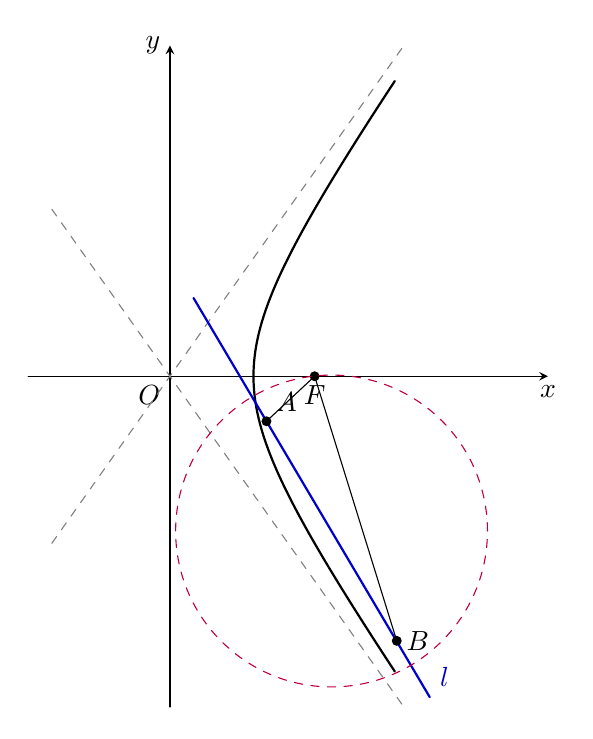
\begin{tikzpicture}[scale=1.5, >=stealth, line cap=round, line join=round]
  % 坐标轴
  \draw[->] (-1.2, 0) -- (3.2, 0) node[below] {$x$};
  \draw[->] (0, -2.8) -- (0, 2.8) node[left] {$y$};
  \node[below left] at (0, 0) {$O$};

  % 渐近线
  \draw[dashed, thin, gray] (-1.0, -1.414) -- (2.0, 2.828);
  \draw[dashed, thin, gray] (-1.0, 1.414) -- (2.0, -2.828);

  % 双曲线右支 2x^2 - y^2 = 1 => x = sqrt((1 + y^2)/2)
  \draw[thick, smooth, domain=-2.5:2.5, samples=60] 
    plot ({sqrt((1 + \x*\x)/2)}, \x);

  % 焦点 F(sqrt(6)/2, 0) ≈ (1.225, 0)
  \coordinate (F) at (1.2247, 0);
  \fill (F) circle (1.2pt) node[below] {$F$};

  % 直线 y = kx + 1，k = -(6 + sqrt(6))/5 ≈ -1.6899
  \coordinate (A) at (0.817, -0.381);
  \coordinate (B) at (1.92, -2.24);
  \draw[domain=0.2:2.2, smooth, thick, blue!80!black] 
    plot (\x, {-1.6899*\x + 1}) node[above right] {$l$};

  \fill (A) circle (1.2pt) node[above right] {$A$};
  \fill (B) circle (1.2pt) node[right] {$B$};

  % 直径圆中心与圆
  \coordinate (M) at (1.368, -1.31);
  \draw[dashed, thin, purple] (M) circle (1.32);

  \draw[thin] (A) -- (F) -- (B);
\end{tikzpicture}
